%% LyX 2.0.7.1 created this file.  For more info, see http://www.lyx.org/.
%% Do not edit unless you really know what you are doing.
\documentclass[english]{sig-alternate-2013}
\usepackage[T1]{fontenc}
\usepackage[latin9]{inputenc}
\usepackage{verbatim}
\usepackage{graphicx}

\makeatletter

%%%%%%%%%%%%%%%%%%%%%%%%%%%%%% LyX specific LaTeX commands.
%% A simple dot to overcome graphicx limitations
\newcommand{\lyxdot}{.}


%%%%%%%%%%%%%%%%%%%%%%%%%%%%%% User specified LaTeX commands.
\usepackage{subfigure}
\usepackage{algorithmic}
\DeclareMathOperator*{\argmax}{arg\,max}

\makeatother

\usepackage{babel}
\begin{document}
%\title{An Evaluation of Query Expansion for Patent Prior Art Search}
%\title{Query Expansion Methods for Patent Prior Art Search with Partial Applications}
\title{Query Expansion Methods for Prior Art Search with Partial Patent Applications}
%\title{ A Study of Query Reformulation for Patent Prior Art Search}
\numberofauthors{1}
\author{
\alignauthor
}
\newtheorem{proposition}{Proposition}
\maketitle

\begin{abstract}
Patents are used by entities to legally protect their inventions and
represent a multi-billion dollar industry of licensing and litigation.
In 2012, 276,788 patent applications were approved in the US alone
-- a number that has doubled in the past 15 years. While much of the
literature inspired by the evaluation framework of the CLEF-IP competition
has aimed to assist patent examiners in assessing prior art for complete
patent applications, less of this work has focused on patent search
with shorter queries representing (partial) titles, abstract, or claims
to help inventors assess the patentability of their ideas prior to
writing a full application. In this paper, we focus on the latter
task and specifically on query expansion methods that are targeted
for patent prior art search. We propose query expansion methods that
exploit the specific structure of patent documents as well as methods
aimed to improve recall with a limited set of query expansion terms.
We demonstrate that our methods improve both general (MAP) and patent-specific
(PRES) evaluation metrics for prior art search performance on standardized
datasets of CLEF-IP.
\end{abstract}

\vspace{1mm}
\noindent
{\bf Categories and Subject Descriptors:} H.3.3 {[Information Systems]}: {Information Storage and Retrieval, Information Search and Retrieval}

\vspace{1mm}
\noindent
{\bf General Terms:} Algorithms, Experimentation.

\vspace{1mm}
\noindent
{\bf Keywords:} Query Expansion, Patent Search.


\section{Introduction}

\noindent %Patents are used by entities to legally protect their inventions and
%represent a multi-billion dollar industry of licensing and litigation.
%In 2012, 276,788 patent applications were approved in the US alone
%-- a number that has doubled in the past 15 years. 
Patent prior art search involves finding previously granted patents
that may be relevant to a new patent application. The objective and
challenges of standard formulations of patent prior art search are
different from those of standard text and web search since~\cite{Magdy2012}:
(i) queries are full patent applications, which consist of documents
with hundreds of words organized into several sections, while queries
in text and web search constitute only a few words; (ii) patent prior
art search is a recall-oriented task, where the primary focus is to
retrieve all relevant documents at early ranks, in contrast to text
and web search that are precision-oriented. %where the primary goal is to retrieve a subset of relevant documents
%at early ranks.


While much of the literature inspired by the evaluation framework
of the CLEF-IP competition has aimed to assist patent examiners in
assessing prior art for complete patent applications, less work has
focused on assessing the patentability of inventions before writing
a full patent application. Prior art search with shorter queries that
represent unfinished patent applications is certainly desirable, since
writing a full application is time-consuming and costly, especially
if lawyers are hired to assist. However prior art search with partial
applications is much different than queries with a full application
-- namely because the queries are much shorter and represent only
parts of a patent application. 

%%%%%%%%%%%%%%%%%%%%%%%%%%%%%%%%%%%%%%%%%%%%%%%%%%%%%%%%%%%%%%%%%%%%%
\begin{figure}[t!]
\begin{centering}
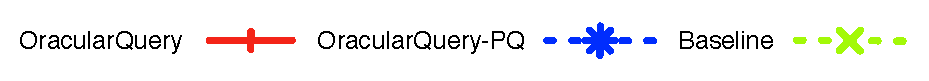
\includegraphics[width=3.5cm,bb = 0 0 200 100, draft, type=eps]{../../Downloads/SIGIR14/img/legend.eps} 
\par\end{centering}

\subfigure[Title query.]{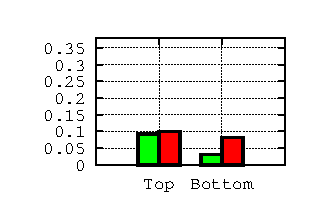
\includegraphics[width=2.75cm]{Results-CIKM2014/jaccard-qTitle-CLEF-IP2010}}\subfigure[Abstract query.]{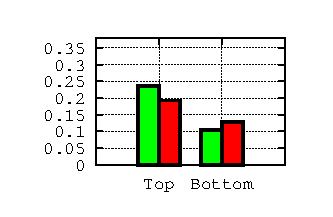
\includegraphics[width=2.75cm]{Results-CIKM2014/jaccard-qAbstract-CLEF-IP2010}}\subfigure[Claims query.]{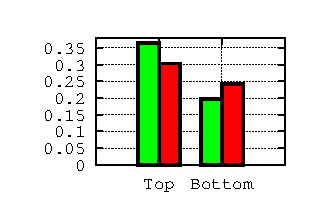
\includegraphics[width=2.75cm]{Results-CIKM2014/jaccard-qClaims-CLEF-IP2010}}
\vspace{-3mm}
 \caption{{\footnotesize{}Average Jaccard similarity of (ir)relevant documents
with the result sets for different queries. }}


{\footnotesize{}%different queries (representing the title, abstract, or claims of a patent application)
%and the labeled (ir)relevant documents for the best (top) and worst (bottom) performing
%queries from CLEF-IP 2010 w.r.t. MAP.}
\label{fig:FailureAnalysis} \vspace{-1mm}
 }
\end{figure}


%%%%%%%%%%%%%%%%%%%%%%%%%%%%%%%%%%%%%%%%%%%%%%%%%%%%%%%%%%%%%%%%%%%%%


To assess the difficulty of querying with partial patent applications
(such as the title, abstract, or claims sections), we refer to Figure~\ref{fig:FailureAnalysis}.
Here we show an analysis of the average Jaccard similarity (fraction
of overlapping terms after removing patent-specific stopwords) between
different queries (representing the title, abstract, or claims of
a patent application) and the labeled relevant (all) and irrelevant
documents (top 10 non-relevant documents ranked by BM25). We show
results for the top 100 and bottom 100 queries of CLEP-IP 2010 evaluated
according to MAP. There are three notable trends here: (i) term overlap
increases from title to query to claims since the query size grows
accordingly; (ii) the bottom 100 performing queries tend to have much
smaller term overlap with the relevant documents than the top 100
queries; and (iii) the best overlap for any relevant document set
for any set of queries is less than one in four terms. While these
results suggest the claims section may be the best part of a partial
patent application to use for a query, there is still significant
room for improving the overlap of query terms with the relevant documents,
which suggests an investigation of \emph{query expansion}~\cite{Efthimiadis1996}
methods. % to augment a query
%with additional terms likely to occur in relevant documents.
%A term mismatch between
%full patent applications and their relevant documents was also found
%by \cite{Magdy2012}. To overcome the term mismatch query expansion
%seems an appropriate solution.
This is the task we evaluate in the rest of the paper.

% Yes we do better with claims, but it takes more effort to write them.


% this problem by using query expansion
%methods with queries representing sections of patent applications
%such as title, abstract and claims. Our contributions are the following:
%(i) an approach for diverse patent query expansion; (ii) a study about
%query expansion methods that exploits the patent specific structure;
%(iii) a study about the use of different patents' fields as source
%of query expansion terms; (iv) an intensive evaluation of these methods
%using both general (MAP) and patent-specific (PRES) \cite{Magdy2010a}
%evaluation metrics for prior art search on the standardized CLEF-IP
%datasets.
%The rest of this paper is organized as follows: in Section \ref{sec:relatedworks},
%we present the related work. Section \ref{sec:approach} introduces
%our approach for diverse patent query expansion. Experiments are discussed
%in Section \ref{sec:eval}. We conclude and provide some future directions
%in Section \ref{sec:conclusion}.



\section{Query Expansion for Patents}


\subsection{General Framework}

\label{sec:framework}

Query expansion (QE)~\cite{Efthimiadis1996} is an approach that
(automatically) adds terms to an initial query in order to improve
retrieval performance. In exploring QE for patent search with partial
patent applications, there are many configuration options and associated
questions that we can consider: 
\begin{description}
\item [{Query type:}] We consider a partial patent application to consist
of either the title, the abstract, or the claims section%
\footnote{We assume the description section has not been written since this
is tantamount to writing a full patent application.%
} and allow one to query with each. %\footnote{A query is always
 %evaluated against the full content (title, abstract, claims,
 %description) of granted patent applications since it is sensible
 %to make use of all available content.}  
 A critical question is what part of a partial application an inventor
should write to obtain the best search results? 
\item [{Query expansion source:}] We can consider the title, abstract,
claims, and description section as different QE term sources and ask
which section offers the best source of expansion terms? E.g., are
the title words of particularly high value as expansion terms? 
\item [{Relevance model:}] For initial retrieval of documents in the \emph{pseudo-relevant}
feedback set (PRF) --- often used to generate the terms for QE ---
and subsequent re-retrieval with an expanded term set, there are various
options for the relevance ranking model. In this work, we explore
a probabilistic approach represented by the popular BM25~\cite{Robertson1993}
algorithm as well as a vector space model approach as represented
by TF-IDF~\cite{Salton1975}. A natural question is which relevance
model works best for QE for patent prior art search? 
\item [{Term selection method:}] Once we have identified a query expansion
source, we may consider different methods of selecting terms for expansion.
A standard method for term selection is based on the Rocchio~\cite{Salton1971}
approach, but in the next subsection, we introduce an alternate term
selection method intended to address the high-recall nature of patent
prior art search. Then a natural question to ask is which term expansion
method works best, and with which expansion source and retrieval model? 
\end{description}
Before we proceed to evaluate the above questions, we first define
a novel term selection method to address a potential deficiency of
Rocchio as used in practice for high-recall search that we term MMRQE.


\subsection{MMR Query Expansion (MMRQE)}

% The following is a reasonable argument, but could be refuted by
% reviewers... term coverage and recall are more direct and simple
% arguments.


%Moreover, in contrast to scientific and technical writers, patent
%writers tend to generalize and maximize the scope of what is protected
%by a patent, and try to make sure that finding any relevant prior
%work by the patent examiner is a hard job. This leads to the usage
%of unusual expressions that makes finding similar patents a difficult
%task. This specificity of patents content led us to explore a method
%of term diversification selection for query expansion (the diversification
%here arise to select terms not only similar to the query to avoid
%the effect of its ambiguity). More specifically, we propose a new
%algorithm for query expansion based on the Maximal Marginal Relevance
%(MMR) \cite{Carbonell1998} method, which is an approach for result
%set diversification. We refer to our method from now on as MMRQE,
%which we define as a query expansion method that selects terms by
%carrying out a trade-off between diversification and similarity to
%the query.


While space precludes a full discussion, we remark that as a term
selection method in QE, Rocchio derives a score for each potential
query expansion term and in practice, the top-$k$ scoring terms (often
for $k\ll200$) are used to expand the query and are weighted according
to their Rocchio score during the second stage of retrieval. The caveat
of this approach is that given a limited budget of $k$ expansion
terms, there is no inherent guarantee that these terms ``cover''
all documents in the pseudo-relevant set. It seems that what we are
asking for then is a method of ``diverse'' term selection --- something
like the \emph{maximal marginal relevance} (MMR)~\cite{Carbonell1998}
algorithm for result set diversification, but rather than for diverse
document selection as typically used, we intend to use it here for
diverse term selection. 

%%%%%%%%%%%%%%%%%%%%%%%%%%%%%%%%%%%%%%%%%%%%%%%%%%%%%%%%%%%%%%%%%%%%%
\begin{figure}[t!]
\begin{centering}
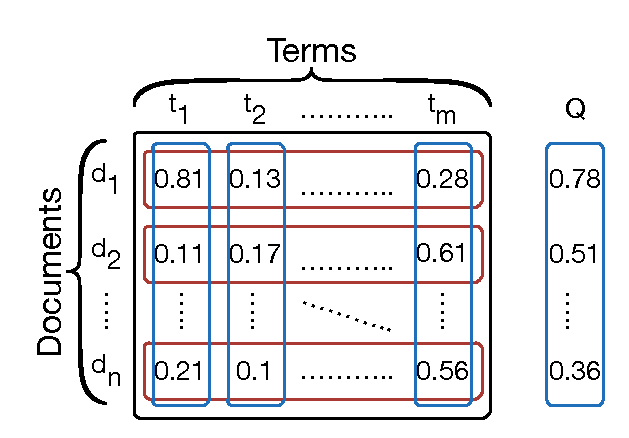
\includegraphics[width=6cm]{img/matrix} 
\par\end{centering}

\vspace{-1mm}
 \caption{Notation used in MMRQE.}


\label{fig:notation} \vspace{-1mm}
 
\end{figure}


%%%%%%%%%%%%%%%%%%%%%%%%%%%%%%%%%%%%%%%%%%%%%%%%%%%%%%%%%%%%%%%%%%%%%


We begin our formal description of MMRQE by first defining some necessary
notation. MMRQE takes as input a pseudo-relevant feedback set of $n$
documents (PRF), which is obtained after a retrieval for the initial
query. From the PRF set, we build a document-term matrix of $n$ documents
and $m$ terms as shown in Figure~\ref{fig:notation}, which uses
a TF-IDF weighting for each document vector (row $d_{i}$ for $1\leq i\leq n$).
However, as we will see shortly, the view that will be important for
us in this work is instead the term vector (column $t_{j}$ for $1\leq j\leq m$).
To represent the query $Q$ column vector in Figure~\ref{fig:notation}
having a numerical entry for every document $d_{i}$, we found that
computing the BM25 or TF-IDF score between each document $d_{i}$
and the query provided the best performance (in our experiments, the
score used is given by the indicated relevance model).

Given a query representation $Q$, we aim to select an optimal subset
of $k$ terms $T_{k}^{*}\subset D$ (where $|T_{k}^{*}|=k$ and $k\ll|m|$)
relevant to $Q$ but inherently different from each other (i.e., diverse).
This can be achieved by building $T_{k}^{*}$ in a greedy manner by
choosing the next optimal term $t_{k}^{*}$ given the previous set
of optimal term selections $T_{k-1}^{*}=\{t_{1}^{*},\ldots,t_{k-1}^{*}\}$
(assuming $T_{0}^{*}=\emptyset$) using the MMR diverse selection
criterion: 

\[
t_{k}^{*}=\argmax_{t_{k}\notin T_{k-1}^{*}}\hspace{-0.3mm}[\lambda\cos(Q,t_{k})-\hspace{-0.3mm}(1-\lambda)\max_{t_{j}\in T_{k-1}^{*}}\cos(t_{j},t_{k})]
\]


Here, the first cosine similarity term measures relevance between
the query $Q$ and possible expansion term $t_{k}$ while the second
term penalizes the possible expansion term according to it's cosine
similarity with any currently selected term in $T_{k-1}^{*}$. The
parameter $\lambda\in[0,1]$ trades off relevance and diversity and
we found $\lambda=0.5$ to generally provide the best results in our
experiments.

The key insight we want to conclude this section with is simply that
MMRQE does not select expansion terms independently as in practical
usage of Rocchio, but rather it selects terms that have uncorrelated
usage patterns across documents, thus hopefully encouraging diverse
term selection that covers more documents for a fixed expansion budget
$k$ and ideally, higher recall. To see if this is true (among other
questions), we now proceed to empirical evaluation.

%%%%%%%%%%%%%%%%%%%%%%%%%%%%%%%%%%%%%%%%%%%%%%%%%%%%%%%%%%%%%%%%%%
%%                Gabriela has edited from here
%%%%%%%%%%%%%%%%%%%%%%%%%%%%%%%%%%%%%%%%%%%%%%%%%%%%%%%%%%%%%%%%%%


\begin{comment}

\section{MMR Query Reduction (MMR QR)}

Given a query representation $Q$, we aim to select an optimal subset
of $k$ terms $T_{k}^{*}\subset Q$ (where $|T_{k}^{*}|=k$ and $k<|Q|$)
relevant to $Q$ but inherently different from each other (i.e., diverse).
This can be achieved by building $T_{k}^{*}$ in a greedy manner by
choosing the next optimal term $t_{k}^{*}$ given the previous set
of optimal term selections $T_{k-1}^{*}=\{t_{1}^{*},\ldots,t_{k-1}^{*}\}$
(assuming $T_{0}^{*}=\emptyset$) using an adaptation of the MMR diverse
selection criterion:

\[
t_{k}^{*}=\argmax_{t_{k}\notin T_{k-1}^{*}}\hspace{-0.3mm}[\lambda\cos(Q,t_{k})-\hspace{-0.3mm}(1-\lambda)\max_{t_{j}\in T_{k-1}^{*}}\cos(t_{j},t_{k})]
\]


Here, the first cosine similarity part (i) aims to select a term $t_{k}$
that will save the current results of the complete query $Q$, while
the second part (ii) penalizes the term according to it's cosine similarity
with any currently selected term in $T_{k-1}^{*}$. The parameter
$\lambda\in[0,1]$ trades off relevance and diversity.
\end{comment}



\section{Experimental results}

\label{results}

We used the Lucene IR System to index the English subset of CLEF-IP
2010 dataset%
\footnote{\texttt{http://www.ifs.tuwien.ac.at/~clef-ip/}%
}~\cite{Piroi2011} with the default stemming, standard stop-word
removal and patent-specific stop-words, as described in \cite{Magdy2012}.
The English test set corresponds to 1303 topics. In our implementation,
each section of a patent application (title, abstract, claims, and
description) are indexed in separate fields. When a query is performed,
all fields in the index are targeted. As recommended in \cite{Magdy2012}
and confirmed in our own experimentation (not shown due to lack of
space), best QE performance results are obtained when using few documents
in the PRF set (in our case, the top five gave the best results). 

We carry out comprehensive experiments along the four dimensions outlined
in~\ref{sec:framework} with the following specific options: 
\begin{itemize}
\item \textbf{Query type:} $\{\mathrm{Title},\mathrm{Abstract},\mathrm{Claims}\}$ 
\item \textbf{Query expansion source:} $\{\mathrm{Title},\mathrm{Abs.},\mathrm{Claims},\mathrm{Descrip.}\}$ 
\item \textbf{Relevance model:} $\{\mathrm{BM25},\mbox{Vector-space Model (VSM)}\}$ 
\item \textbf{Term selection method:} $\{\mathrm{Rocchio},\mathrm{MMRQE}\}$ 
\end{itemize}
e include one additional QE baseline motivated by \cite{Mahdabi2013},
where the text definitions of the International Patent Classification
(IPC) codes assigned to a patent application are used as a source
for query expansion --- this is denoted as \textbf{Class Code}.

The relevance model and term selection options give us four QE algorithms
to evaluate. When MMRQE is used in combination with the VSM, the additional
terms use the weights provided by the Rocchio method, whereas when
using MMRQE and Rocchio with BM25, there is no need to weight the
terms. For both MMRQE and Rocchio, their parameters were fixed to
their optimal values, which were estimated using the CLEF-IP training
queries.

We report MAP and PRES on the top 1000 results. PRES \cite{Magdy2012}
is a metric that combines recall with the quality of ranking and weights
relevant documents lower in the ranking more highly than MAP.

Figures~\ref{fig:MAP-CLEF2010} and~\ref{fig:PRES-CLEF2010} show
the performance across different queries and sources of expansion
respectively in terms of MAP and PRES for CLEF-IP 2010 for different
numbers of expanded terms $k$ on the x-axis (with $k=0$ using no
QE, just the baseline retrieval model). From these results, we observe
the best section to use for \emph{both} querying and the source of
query expansion terms is the claims section (see the bottom line of
Figures~\ref{fig:MAP-CLEF2010} and~\ref{fig:PRES-CLEF2010}). We
attribute this to the fact that the claims section has more content
along with more terms relevant to specific details of the patent,
since the core of the invention is described therein. Very similar
overall results are obtained for CLEF-IP 2011 and for space reasons
we cannot show them here. %only
%show the results for the claims queries in
%Figures~\ref{fig:MAP-CLEF2011} and \ref{fig:PRES-CLEF2011}.


We observed that query expansion is typically more useful for short
queries (i.e. title, abstract), indicating that in the very preliminary
stages of the patent application process, QE is important. %whereas for the whole patent application (including the description
%section), query expansion may hurt the performance
%\cite{Itoh2004,Magdy2011}; {\color{red}Gaby said: not sure if we want
%  to keep these references here!, since we are not showing that in the
%  figures.}  
We also notice that when dealing with more complex queries such as
claims, MMRQE is more effective than Rocchio, which suggest that diverse
term selection is not crucial for short queries.

%The best sources for expansion are the abstract and claims sections (see graphs (j) and (k) from Figures \ref{fig:MAP-CLEF2010}, \ref{fig:PRES-CLEF2010},
%\ref{fig:MAP-CLEF2011} and \ref{fig:PRES-CLEF2011})
%Note that the title is not a good source of expansion
%(see the first column from Figures \ref{fig:MAP-CLEF2010}, \ref{fig:PRES-CLEF2010},
%\ref{fig:MAP-CLEF2011} and \ref{fig:PRES-CLEF2011}).
%We attribute this to the short length and poor term variability of the title.


% ***


It is interesting to notice that the description is not either a good
source for expansion, since it may contain more general terms that
may hurt the performance (see the fourth column from Figures \ref{fig:MAP-CLEF2010}
and \ref{fig:PRES-CLEF2010}). %,
%\ref{fig:MAP-CLEF2011}, and \ref{fig:PRES-CLEF2011}). 
Finally, we observed that using the IPC definitions as a source of
expansion, as suggested by \cite{Mahdabi2013}, gave poor performance
(see Class Code curve along the Figures).

Regarding the best term selection method, we conclude that Rocchio
is better in retrieving patents since it gives best performance for
PRES in general, while MMRQE is better for ranking since it gives
better performance for MAP.

%\begin{figure*}[t]
%\begin{centering}
%\subfigure[{\tiny Query Claims \& source Title.}]{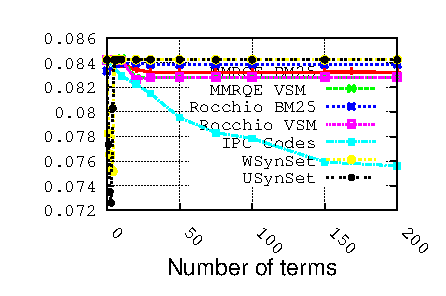
\includegraphics[width=4.3cm]{Results-SIGIR2014/qClaims-sTitle_MAP_2011}}\subfigure[{\tiny Query Claims \& source Abstract.}]{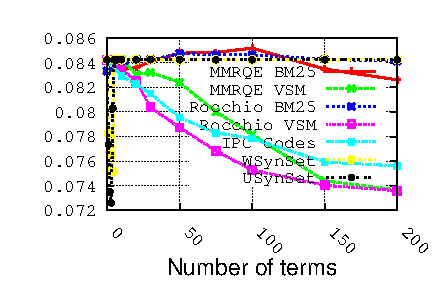
\includegraphics[width=4.3cm]{Results-SIGIR2014/qClaims-sAbstract_MAP_2011}}\subfigure[{\tiny Query Claims \& source Claims.}]{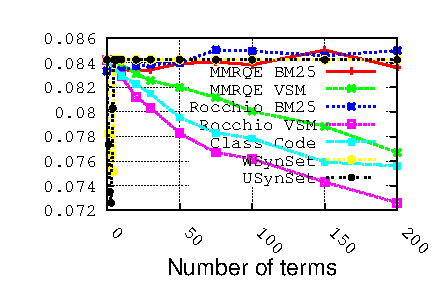
\includegraphics[width=4.3cm]{Results-SIGIR2014/qClaims-sClaims_MAP_2011}}\subfigure[{\tiny Query Claims \& source Descrip.}]{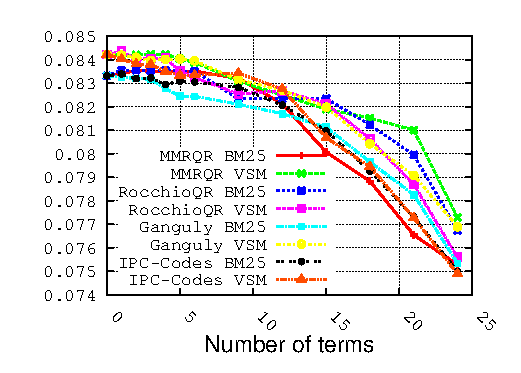
\includegraphics[width=4.3cm]{Results-SIGIR2014/qClaims-sDescription_MAP_2011}}
%\par\end{centering}
%\vspace{-3mm}
%\caption{Mean Average Precision (MAP) on CLEF-2011 (for MMRQE $\lambda=0.5$).}
%\label{fig:MAP-CLEF2011}
%\vspace{-3mm}
%\end{figure*}


%\begin{figure*}
%\begin{centering}
%\subfigure[{\tiny Query Claims \& source Title.}]{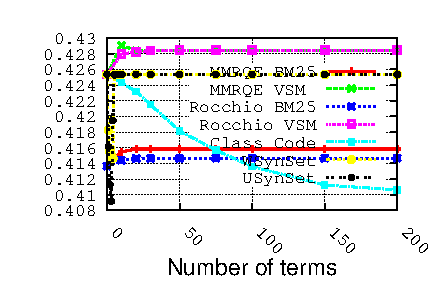
\includegraphics[width=4.3cm]{Results-SIGIR2014/qClaims-sTitle_PRES_2011}}\subfigure[{\tiny Query Claims \& source Abstract.}]{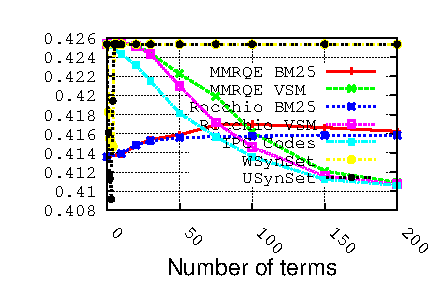
\includegraphics[width=4.3cm]{Results-SIGIR2014/qClaims-sAbstract_PRES_2011}}\subfigure[{\tiny Query Claims \& source Claims.}]{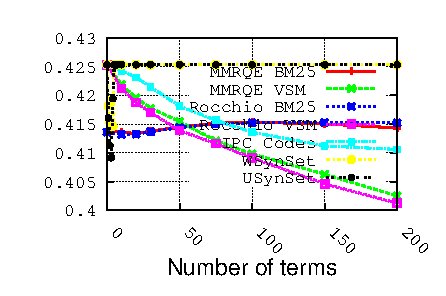
\includegraphics[width=4.3cm]{Results-SIGIR2014/qClaims-sClaims_PRES_2011}}\subfigure[{\tiny Query Claims \& source Descrip.}]{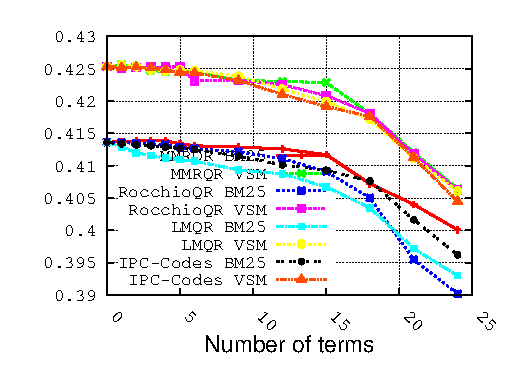
\includegraphics[width=4.3cm]{Results-SIGIR2014/qClaims-sDescription_PRES_2011}}
%\par\end{centering}
%\vspace{-3mm}
%\caption{Patent Retrieval Evaluation Score (PRES) on CLEF-2011 (for MMRQE $\lambda=0.5$).}
%\label{fig:PRES-CLEF2011}
%\vspace{-3mm}
%r\end{figure*}


\begin{figure*}[t]
\begin{centering}
\subfigure[{\tiny Query Title \& source Title.}]{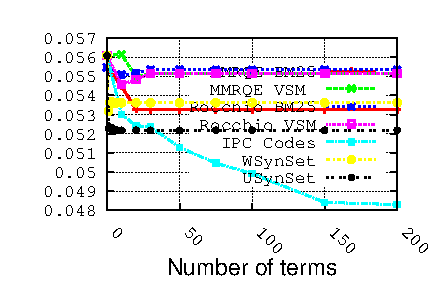
\includegraphics[width=4.3cm]{Results-CIKM2014/qTitle-sTitle_MAP_2010}}\subfigure[{\tiny Query Title \& source Abstract.}]{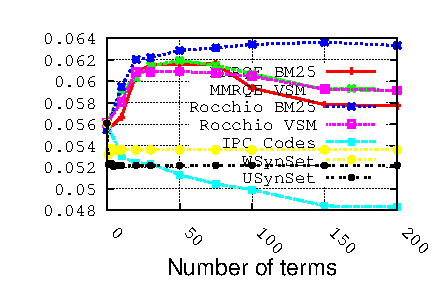
\includegraphics[width=4.3cm]{Results-CIKM2014/qTitle-sAbstract_MAP_2010}}\subfigure[{\tiny Query Title \& source Claims.}]{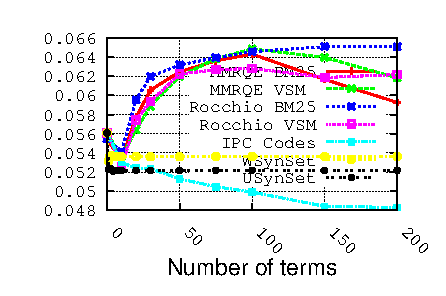
\includegraphics[width=4.3cm]{Results-CIKM2014/qTitle-sClaims_MAP_2010}}\subfigure[{\tiny Query Title \& source Descrip.}]{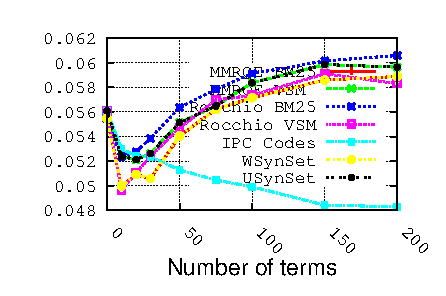
\includegraphics[width=4.3cm]{Results-CIKM2014/qTitle-sDescription_MAP_2010}} 
\par\end{centering}

\begin{centering}
\subfigure[{\tiny Query Abstract \& source Title.}]{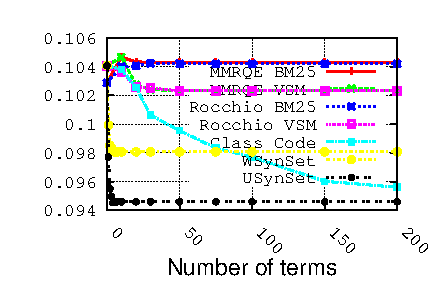
\includegraphics[width=4.3cm]{Results-CIKM2014/qAbstract-sTitle_MAP_2010}}\subfigure[{\tiny Query Abstract \& source Abstract.}]{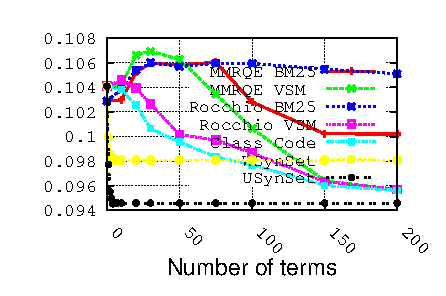
\includegraphics[width=4.3cm]{Results-CIKM2014/qAbstract-sAbstract_MAP_2010}}\subfigure[{\tiny Query Abstract \& source Claims.}]{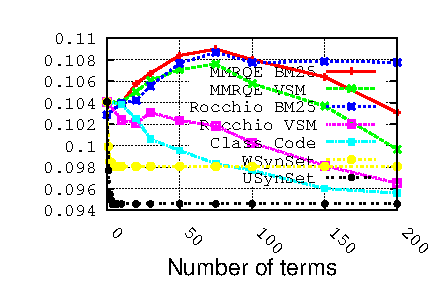
\includegraphics[width=4.3cm]{Results-CIKM2014/qAbstract-sClaims_MAP_2010}}\subfigure[{\tiny Query Abstract \& source Descrip.}]{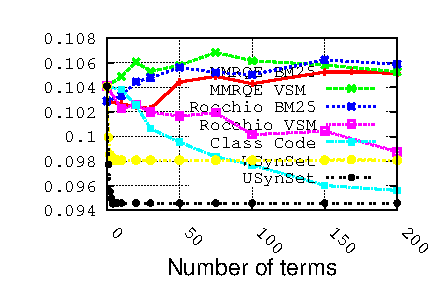
\includegraphics[width=4.3cm]{Results-CIKM2014/qAbstract-sDescription_MAP_2010}} 
\par\end{centering}

\begin{centering}
\subfigure[{\tiny Query Claims \& source Title.}]{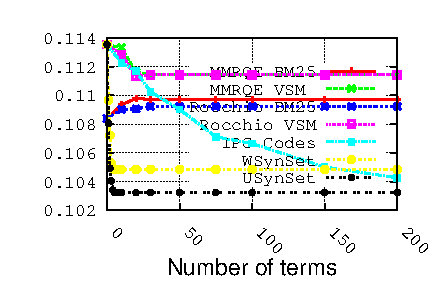
\includegraphics[width=4.3cm]{Results-CIKM2014/qClaims-sTitle_MAP_2010}}\subfigure[{\tiny Query Claims \& source Abstract.}]{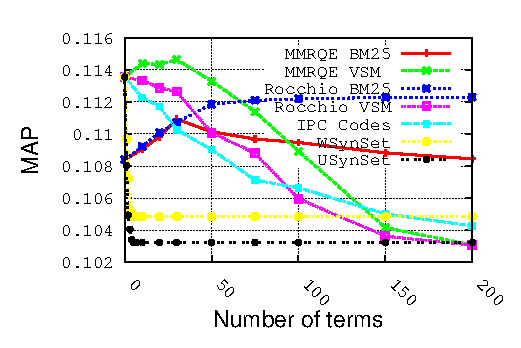
\includegraphics[width=4.3cm]{Results-CIKM2014/qClaims-sAbstract_MAP_2010}}\subfigure[{\tiny Query Claims \& source Claims.}]{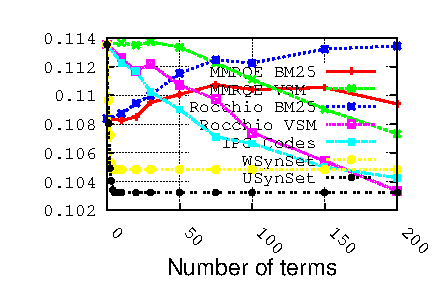
\includegraphics[width=4.3cm]{Results-CIKM2014/qClaims-sClaims_MAP_2010}}\subfigure[{\tiny Query Claims \& source Descrip.}]{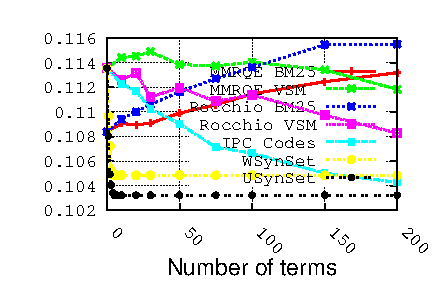
\includegraphics[width=4.3cm]{Results-CIKM2014/qClaims-sDescription_MAP_2010}}
\subfigure[{\tiny Query Descrip \& source Title.}]{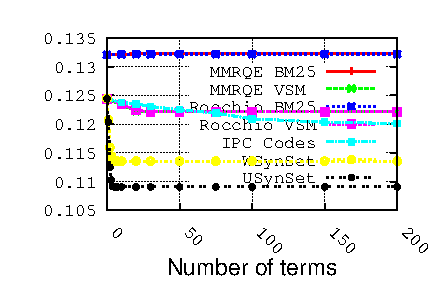
\includegraphics[width=4.3cm]{Results-CIKM2014/qDescription-sTitle_MAP_2010}}\subfigure[{\tiny Query Descrip \& source Abstract.}]{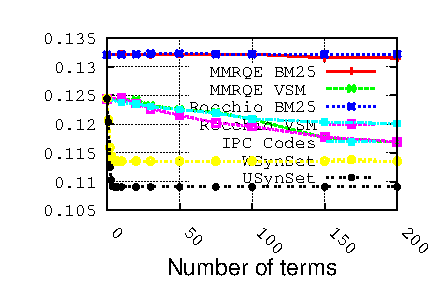
\includegraphics[width=4.3cm]{Results-CIKM2014/qDescription-sAbstract_MAP_2010}}\subfigure[{\tiny Query Descrip \& source Claims.}]{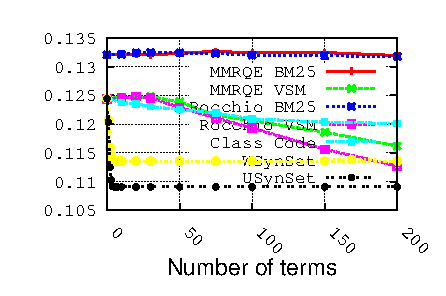
\includegraphics[width=4.3cm]{Results-CIKM2014/qDescription-sClaims_MAP_2010}}\subfigure[{\tiny Query Descrip \& source Descrip.}]{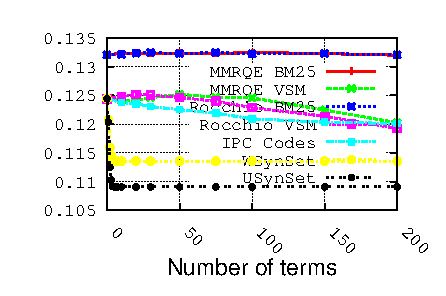
\includegraphics[width=4.3cm]{Results-CIKM2014/qDescription-sDescription_MAP_2010}} 
\par\end{centering}

\caption{Mean Average Precision (MAP) on CLEF-2010 (for MMRQE $\lambda=0.5$).}


\label{fig:MAP-CLEF2010}
\end{figure*}


\begin{figure*}
\begin{centering}
\subfigure[{\tiny Query Title \& source Title.}]{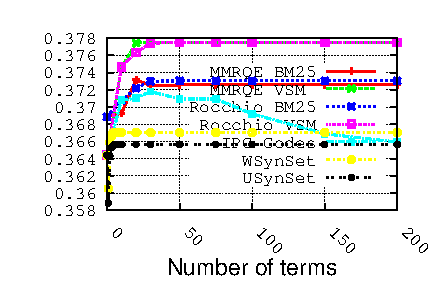
\includegraphics[width=4.3cm]{Results-CIKM2014/qTitle-sTitle_PRES_2010}}\subfigure[{\tiny Query Title \& source Abstract.}]{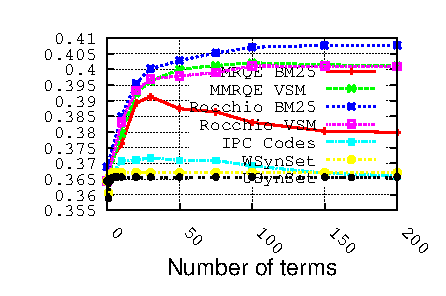
\includegraphics[width=4.3cm]{Results-CIKM2014/qTitle-sAbstract_PRES_2010}}\subfigure[{\tiny Query Title \& source Claims.}]{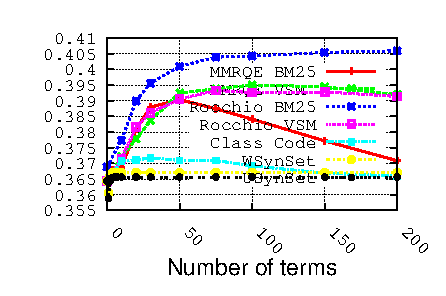
\includegraphics[width=4.3cm]{Results-CIKM2014/qTitle-sClaims_PRES_2010}}\subfigure[{\tiny Query Title \& source Descrip.}]{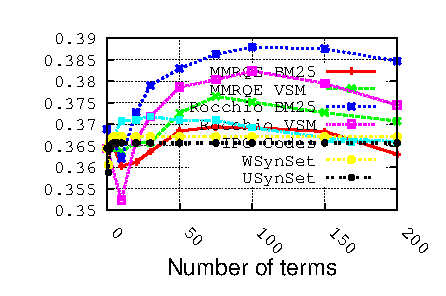
\includegraphics[width=4.3cm]{Results-CIKM2014/qTitle-sDescription_PRES_2010}} 
\par\end{centering}

\begin{centering}
\subfigure[{\tiny Query Abstract \& source Title.}]{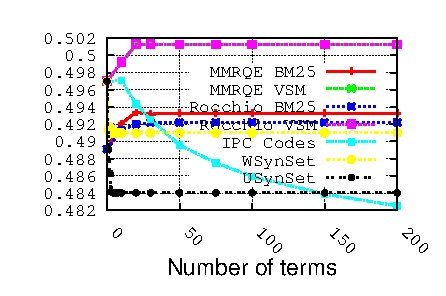
\includegraphics[width=4.3cm]{Results-CIKM2014/qAbstract-sTitle_PRES_2010}}\subfigure[{\tiny Query Abstract \& source Abstract.}]{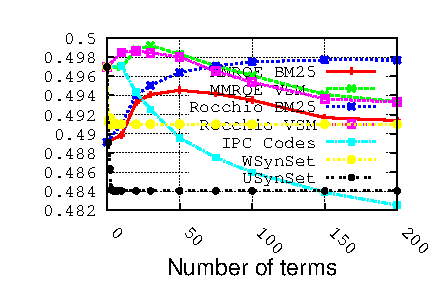
\includegraphics[width=4.3cm]{Results-CIKM2014/qAbstract-sAbstract_PRES_2010}}\subfigure[{\tiny Query Abstract \& source Claims.}]{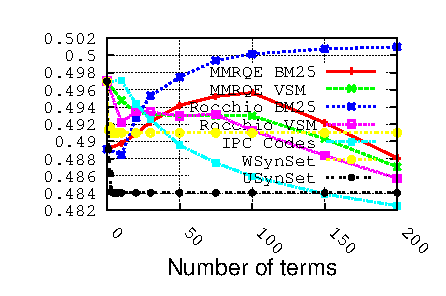
\includegraphics[width=4.3cm]{Results-CIKM2014/qAbstract-sClaims_PRES_2010}}\subfigure[{\tiny Query Abstract \& source Descrip.}]{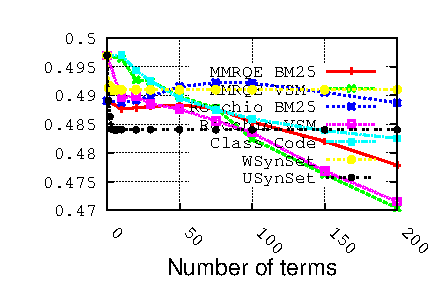
\includegraphics[width=4.3cm]{Results-CIKM2014/qAbstract-sDescription_PRES_2010}} 
\par\end{centering}

\begin{centering}
\subfigure[{\tiny Query Claims \& source Title.}]{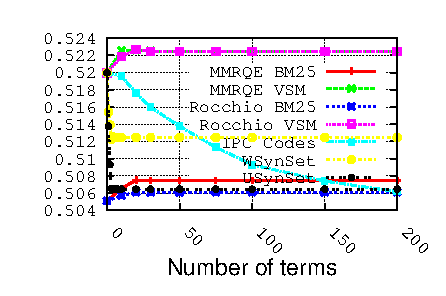
\includegraphics[width=4.3cm]{Results-CIKM2014/qClaims-sTitle_PRES_2010}}\subfigure[{\tiny Query Claims \& source Abstract.}]{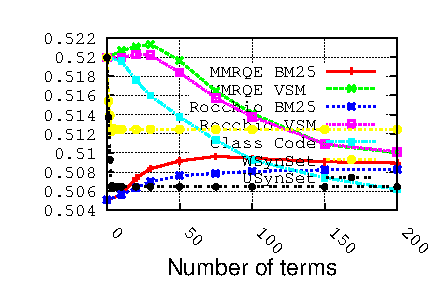
\includegraphics[width=4.3cm]{Results-CIKM2014/qClaims-sAbstract_PRES_2010}}\subfigure[{\tiny Query Claims \& source Claims.}]{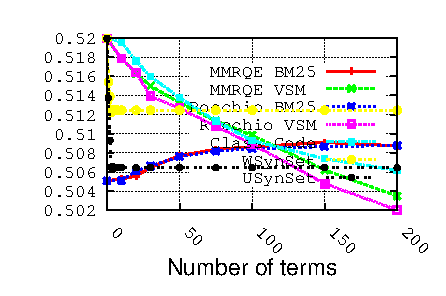
\includegraphics[width=4.3cm]{Results-CIKM2014/qClaims-sClaims_PRES_2010}}\subfigure[{\tiny Query Claims \& source Descrip.}]{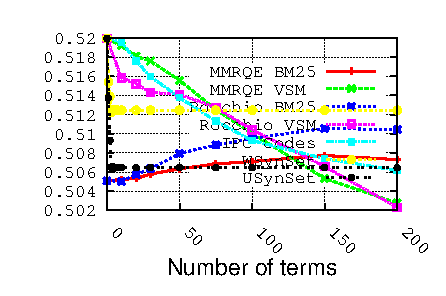
\includegraphics[width=4.3cm]{Results-CIKM2014/qClaims-sDescription_PRES_2010}}
\subfigure[{\tiny Query Descrip \& source Title.}]{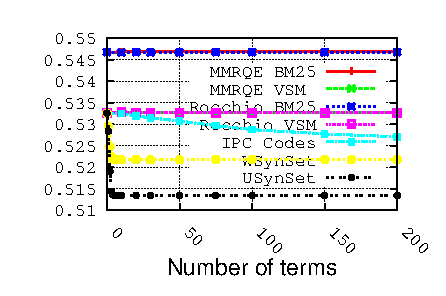
\includegraphics[width=4.3cm]{Results-CIKM2014/qDescription-sTitle_PRES_2010}}\subfigure[{\tiny Query Descrip \& source Abstract.}]{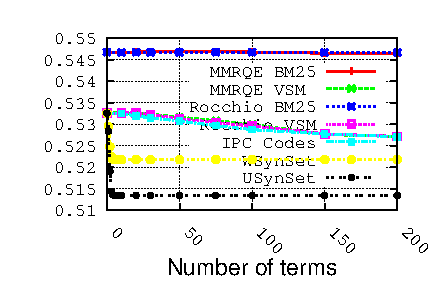
\includegraphics[width=4.3cm]{Results-CIKM2014/qDescription-sAbstract_PRES_2010}}\subfigure[{\tiny Query Descrip \& source Claims.}]{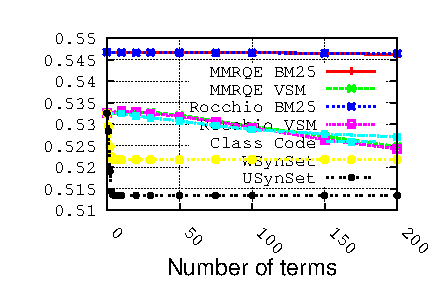
\includegraphics[width=4.3cm]{Results-CIKM2014/qDescription-sClaims_PRES_2010}}\subfigure[{\tiny Query Descrip \& source Descrip.}]{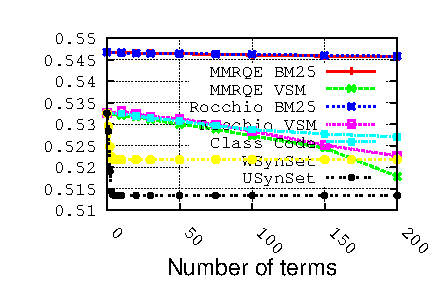
\includegraphics[width=4.3cm]{Results-CIKM2014/qDescription-sDescription_PRES_2010}} 
\par\end{centering}

\caption{Patent Retrieval Evaluation Score (PRES) on CLEF-2010 (for MMRQE $\lambda=0.5$).}


\label{fig:PRES-CLEF2010} 
\end{figure*}
\begin{comment}
\begin{figure*}[t]
\begin{centering}
\subfigure[{\tiny Query Title \& source Title.}]{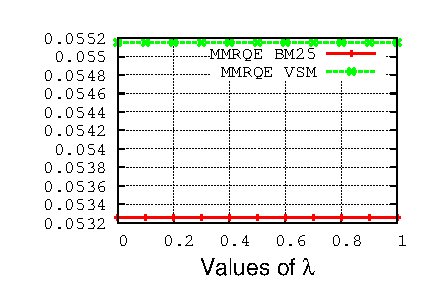
\includegraphics[width=4.3cm]{Results-CIKM2014-lambda/qTitle-sTitle_MAP_2010.eps}}\subfigure[{\tiny Query Title \& source Abstract.}]{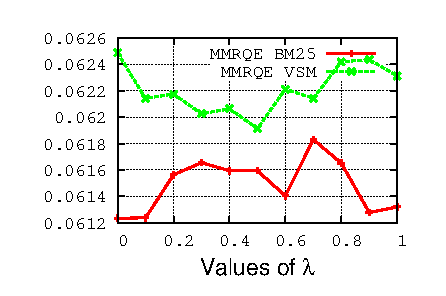
\includegraphics[width=4.3cm]{Results-CIKM2014-lambda/qTitle-sAbstract_MAP_2010.eps}}\subfigure[{\tiny Query Title \& source Claims.}]{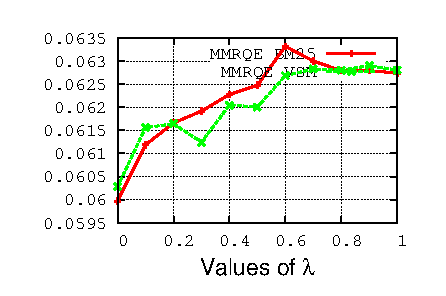
\includegraphics[width=4.3cm]{Results-CIKM2014-lambda/qTitle-sClaims_MAP_2010.eps}}\subfigure[{\tiny Query Title \& source Descrip.}]{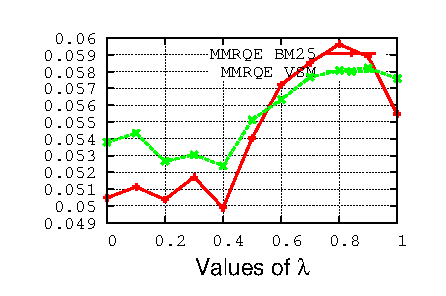
\includegraphics[width=4.3cm]{Results-CIKM2014-lambda/qTitle-sDescription_MAP_2010.eps}} 
\par\end{centering}

\begin{centering}
\subfigure[{\tiny Query Abstract \& source Title.}]{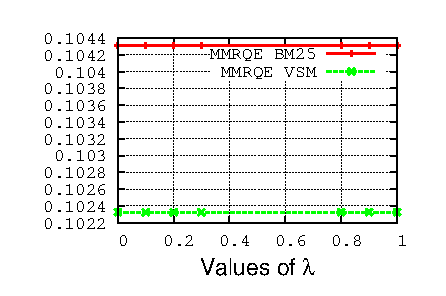
\includegraphics[width=4.3cm]{Results-CIKM2014-lambda/qAbstract-sTitle_MAP_2010.eps}}\subfigure[{\tiny Query Abstract \& source Abstract.}]{\includegraphics[width=4.3cm]{Results-CIKM2014-lambda/qAbstract-sAbstract_MAP_2010.eps}}\subfigure[{\tiny Query Abstract \& source Claims.}]{\includegraphics[width=4.3cm]{Results-CIKM2014-lambda/qAbstract-sClaims_MAP_2010.eps}}\subfigure[{\tiny Query Abstract \& source Descrip.}]{\includegraphics[width=4.3cm]{Results-CIKM2014-lambda/qAbstract-sDescription_MAP_2010.eps}} 
\par\end{centering}

\begin{centering}
\subfigure[{\tiny Query Claims \& source Title.}]{\includegraphics[width=4.3cm]{Results-CIKM2014-lambda/qClaims-sTitle_MAP_2010.eps}}\subfigure[{\tiny Query Claims \& source Abstract.}]{\includegraphics[width=4.3cm]{Results-CIKM2014-lambda/qClaims-sAbstract_MAP_2010.eps}}\subfigure[{\tiny Query Claims \& source Claims.}]{\includegraphics[width=4.3cm]{Results-CIKM2014-lambda/qClaims-sClaims_MAP_2010.eps}}\subfigure[{\tiny Query Claims \& source Descrip.}]{\includegraphics[width=4.3cm]{Results-CIKM2014-lambda/qClaims-sDescription_MAP_2010.eps}} 
\par\end{centering}

\caption{Mean Average Precision (MAP) on CLEF-2010 (for 50 expansion terms).}
\end{figure*}


\begin{figure*}
\begin{centering}
\subfigure[{\tiny Query Title \& source Title.}]{\includegraphics[width=4.3cm]{Results-CIKM2014-lambda/qTitle-sTitle_PRES_2010.eps}}\subfigure[{\tiny Query Title \& source Abstract.}]{\includegraphics[width=4.3cm]{Results-CIKM2014-lambda/qTitle-sAbstract_PRES_2010.eps}}\subfigure[{\tiny Query Title \& source Claims.}]{\includegraphics[width=4.3cm]{Results-CIKM2014-lambda/qTitle-sClaims_PRES_2010.eps}}\subfigure[{\tiny Query Title \& source Descrip.}]{\includegraphics[width=4.3cm]{Results-CIKM2014-lambda/qTitle-sDescription_PRES_2010.eps}} 
\par\end{centering}

\begin{centering}
\subfigure[{\tiny Query Abstract \& source Title.}]{\includegraphics[width=4.3cm]{Results-CIKM2014-lambda/qAbstract-sTitle_PRES_2010.eps}}\subfigure[{\tiny Query Abstract \& source Abstract.}]{\includegraphics[width=4.3cm]{Results-CIKM2014-lambda/qAbstract-sAbstract_PRES_2010.eps}}\subfigure[{\tiny Query Abstract \& source Claims.}]{\includegraphics[width=4.3cm]{Results-CIKM2014-lambda/qAbstract-sClaims_PRES_2010.eps}}\subfigure[{\tiny Query Abstract \& source Descrip.}]{\includegraphics[width=4.3cm]{Results-CIKM2014-lambda/qAbstract-sDescription_PRES_2010.eps}} 
\par\end{centering}

\begin{centering}
\subfigure[{\tiny Query Claims \& source Title.}]{\includegraphics[width=4.3cm]{Results-CIKM2014-lambda/qClaims-sTitle_PRES_2010.eps}}\subfigure[{\tiny Query Claims \& source Abstract.}]{\includegraphics[width=4.3cm]{Results-CIKM2014-lambda/qClaims-sAbstract_PRES_2010.eps}}\subfigure[{\tiny Query Claims \& source Claims.}]{\includegraphics[width=4.3cm]{Results-CIKM2014-lambda/qClaims-sClaims_PRES_2010.eps}}\subfigure[{\tiny Query Claims \& source Descrip.}]{\includegraphics[width=4.3cm]{Results-CIKM2014-lambda/qClaims-sDescription_PRES_2010.eps}} 
\par\end{centering}

\caption{Patent Retrieval Evaluation Score (PRES) on CLEF-2010 (for 50 expansion
terms).}


\label{fig:PRES-CLEF2010-1}
\end{figure*}
\end{comment}


\begin{figure*}[t]
\begin{centering}
\subfigure[{Query Title.}]{\includegraphics[width=8cm]{mmrqrResults/qTitle-sDescription_MAP_2010}}\subfigure[{Query Abstract.}]{\includegraphics[width=8cm]{mmrqrResults/qAbstract-sDescription_MAP_2010}}
\par\end{centering}

\begin{centering}
\subfigure[{Query Claims.}]{\includegraphics[width=8cm]{mmrqrResults/qClaims-sDescription_MAP_2010}}
\subfigure[{Query Description.}]{\includegraphics[width=8cm]{mmrqrResults/qDescription-sDescription_MAP_2010}} 
\par\end{centering}

\caption{Mean Average Precision (MAP) for MMRQR on CLEF-2010 (for MMRQE $\lambda=0.8$).}
\end{figure*}


\begin{figure*}
\begin{centering}
\subfigure[{ Query Title.}]{\includegraphics[width=8cm]{mmrqrResults/qTitle-sDescription_PRES_2010}}\subfigure[{Query Abstract.}]{\includegraphics[width=8cm]{mmrqrResults/qAbstract-sDescription_PRES_2010}}
\par\end{centering}

\begin{centering}
\subfigure[{Query Claims.}]{\includegraphics[width=8cm]{mmrqrResults/qClaims-sDescription_PRES_2010}}
\subfigure[{Query Description.}]{\includegraphics[width=8cm]{mmrqrResults/qDescription-sDescription_PRES_2010}} 
\par\end{centering}

\caption{Patent Retrieval Evaluation Score (PRES) for MMRQR on CLEF-2010 (for
MMRQE $\lambda=0.8$).}
\end{figure*}


\begin{comment}
\begin{figure*}[t]
\begin{centering}
\subfigure[{\tiny Query Title \& source Title.}]{\includegraphics[width=4.3cm]{mmrqrResults-lambda/qTitle-sTitle_MAP_2010.eps}}\subfigure[{\tiny Query Title \& source Abstract.}]{\includegraphics[width=4.3cm]{mmrqrResults-lambda/qTitle-sAbstract_MAP_2010.eps}}\subfigure[{\tiny Query Title \& source Claims.}]{\includegraphics[width=4.3cm]{mmrqrResults-lambda/qTitle-sClaims_MAP_2010.eps}}\subfigure[{\tiny Query Title \& source Descrip.}]{\includegraphics[width=4.3cm]{mmrqrResults-lambda/qTitle-sDescription_MAP_2010.eps}} 
\par\end{centering}

\begin{centering}
\subfigure[{\tiny Query Abstract \& source Title.}]{\includegraphics[width=4.3cm]{mmrqrResults-lambda/qAbstract-sTitle_MAP_2010.eps}}\subfigure[{\tiny Query Abstract \& source Abstract.}]{\includegraphics[width=4.3cm]{mmrqrResults-lambda/qAbstract-sAbstract_MAP_2010.eps}}\subfigure[{\tiny Query Abstract \& source Claims.}]{\includegraphics[width=4.3cm]{mmrqrResults-lambda/qAbstract-sClaims_MAP_2010.eps}}\subfigure[{\tiny Query Abstract \& source Descrip.}]{\includegraphics[width=4.3cm]{mmrqrResults-lambda/qAbstract-sDescription_MAP_2010.eps}} 
\par\end{centering}

\begin{centering}
\subfigure[{\tiny Query Claims \& source Title.}]{\includegraphics[width=4.3cm]{mmrqrResults-lambda/qClaims-sTitle_MAP_2010.eps}}\subfigure[{\tiny Query Claims \& source Abstract.}]{\includegraphics[width=4.3cm]{mmrqrResults-lambda/qClaims-sAbstract_MAP_2010.eps}}\subfigure[{\tiny Query Claims \& source Claims.}]{\includegraphics[width=4.3cm]{mmrqrResults-lambda/qClaims-sClaims_MAP_2010.eps}}\subfigure[{\tiny Query Claims \& source Descrip.}]{\includegraphics[width=4.3cm]{mmrqrResults-lambda/qClaims-sDescription_MAP_2010.eps}} 
\par\end{centering}

\caption{Mean Average Precision (MAP) for MMRQR on CLEF-2010.}
\end{figure*}


\begin{figure*}
\begin{centering}
\subfigure[{\tiny Query Title \& source Title.}]{\includegraphics[width=4.3cm]{mmrqrResults-lambda/qTitle-sTitle_PRES_2010.eps}}\subfigure[{\tiny Query Title \& source Abstract.}]{\includegraphics[width=4.3cm]{mmrqrResults-lambda/qTitle-sAbstract_PRES_2010.eps}}\subfigure[{\tiny Query Title \& source Claims.}]{\includegraphics[width=4.3cm]{mmrqrResults-lambda/qTitle-sClaims_PRES_2010.eps}}\subfigure[{\tiny Query Title \& source Descrip.}]{\includegraphics[width=4.3cm]{mmrqrResults-lambda/qTitle-sDescription_PRES_2010.eps}} 
\par\end{centering}

\begin{centering}
\subfigure[{\tiny Query Abstract \& source Title.}]{\includegraphics[width=4.3cm]{mmrqrResults-lambda/qAbstract-sTitle_PRES_2010.eps}}\subfigure[{\tiny Query Abstract \& source Abstract.}]{\includegraphics[width=4.3cm]{mmrqrResults-lambda/qAbstract-sAbstract_PRES_2010.eps}}\subfigure[{\tiny Query Abstract \& source Claims.}]{\includegraphics[width=4.3cm]{mmrqrResults-lambda/qAbstract-sClaims_PRES_2010.eps}}\subfigure[{\tiny Query Abstract \& source Descrip.}]{\includegraphics[width=4.3cm]{mmrqrResults-lambda/qAbstract-sDescription_PRES_2010.eps}} 
\par\end{centering}

\begin{centering}
\subfigure[{\tiny Query Claims \& source Title.}]{\includegraphics[width=4.3cm]{mmrqrResults-lambda/qClaims-sTitle_PRES_2010.eps}}\subfigure[{\tiny Query Claims \& source Abstract.}]{\includegraphics[width=4.3cm]{mmrqrResults-lambda/qClaims-sAbstract_PRES_2010.eps}}\subfigure[{\tiny Query Claims \& source Claims.}]{\includegraphics[width=4.3cm]{mmrqrResults-lambda/qClaims-sClaims_PRES_2010.eps}}\subfigure[{\tiny Query Claims \& source Descrip.}]{\includegraphics[width=4.3cm]{mmrqrResults-lambda/qClaims-sDescription_PRES_2010.eps}} 
\par\end{centering}

\caption{Patent Retrieval Evaluation Score (PRES) for MMRQR on CLEF-2010.}
\end{figure*}
\end{comment}



\section{Related Work}

\label{sec:relatedworks}

%The major contributions in patent search has focused on query formulation, where the objective is to find the best terms to represent a patent application as a query to achieve high retrieval effectiveness by retrieving all possible relevant documents at high ranks \cite{Magdy2012}.


There are a variety of existing query expansion methods that use synonyms
(both from WordNet and automatically generated)~\cite{Magdy2011},
by supervised learning~\cite{Bashir2010}, by IPC codes (a variant
on our baseline approach that additionally uses the citation network
of patents)~\cite{Verma2011}, and a query-specific patent lexicon
based on the definitions of the IPC~\cite{Mahdabi2013}. While our
intention in this paper was to comprehensively evaluate very general
methods for QE using \emph{partial patent applications}; it would
be interesting future work to comprehensively evaluate all of these
patent-specific QE methods with our generic methods for partial patent
application queries.

%Classical query expansion methods has been used for prior art search by 
%Magdy et al. \cite{Magdy2011}, which rely on pseudo-relevance feedback and WordNet as
%source of expansion terms. However, none of these approaches were
%able to achieve a significant improvement over the baseline. Therefore,
%they introduce a novel approach that automatically generates synonym
%sets for terms, and use them as a source of expansion terms, which
%showed significant improvement with respect to the baseline. 
%Also, Bashir et al. \cite{Bashir2010} propose a query expansion with pseudo-relevance
%feedback. Query expansion terms are selected using a using a machine
%learning approach, by picking terms that may have a potential positive
%impact on the retrieval effectiveness. However, this approach can
%be computational expensive, since the presented features are complicated
%to compute, e.g. Pair-wise Terms Proximity features. 
%Verma and Varma \cite{Verma2011} propose a different approach, which instead of using
%the patent text to query, use its International Patent Classification
%(IPC) codes, which are expanded using the citation network. The formed
%query is used to perform an initial search. The results are then re-ranked
%using queries constructed from patent text. Throughout our experiments,
%we concluded that relying on non-patent terms to expand a query, leads to poor retrieval quality.
%Lastly, a more recent work by Mahdabi et al. \cite{Mahdabi2013} propose to combine query reduction and expansion method for prior art search.
%For query reduction, they shorten the query by taking only the first claim since it contains the core of the invention.
%For the query expansion, they built a query-specific patent lexicon based on the definitions of the IPC. Then, 
%the patent lexicon is used to
%select expansion terms that are focused on the reduced query.


%Others investigated query suggestion for patent prior
%art search, which reflect real-life scenario of examiners, who form
%reproducible boolean queries \cite{Adams2011,Azzopardi2010,Kim2011}. 
%In this paper, we focus on generic query expansion methods, but it would be interesting to apply the founded insights 
%to improve patent search specific strategies as the ones just mentioned.


%Finally, also query reduction methods have been applied in order to deal with long queries, which are composed by full patent applications \cite{Ganguly2011,Itoh2003}. Even these methods are interesting, they are not suited to deal with short queries (partial patent applications).



\section{Conclusion }

\label{sec:conclusion}

In this paper we analyzed general QE methods for patent prior art
search with incomplete patent applications. We demonstrated that QE
methods are critical for short queries, that claims are the ideal
section content both to query with and to use as a source of query
expansion terms, and that a new method MMRQE improves QE results in
many cases. Future work can look at more patent-specific methods of
QE for prior art search with partial patent applications and how they
can be integrated with methods like MMRQE.

%We demonstrated that it reasonable to do prior art search 
%with partial applications, especially when combined with query expansion methods. 
%We also found that the patent specific fields are more suited as a source for expansion than other sources.
%We plan to further refine our approach by using
%a term weighting scheme for MMRQE. Other future work direction is to used MMR
%during query reduction to remove terms, which are not diversified
%in the query.




{ \scriptsize

\bibliographystyle{abbrv}
\bibliography{biblio}


}
\end{document}
